\documentclass[conference]{IEEEtran}
\usepackage{graphicx}
\usepackage{amsmath,amssymb}
\usepackage{booktabs}
\usepackage{algorithm}
\usepackage{algpseudocode}

\begin{document}

\title{Cross-Surface Generalization in U-Net Based Crack Segmentation: A Study of Encoder Backbones, Loss Functions, and Classical Preprocessing}

\author{\IEEEauthorblockN{Zawad Ahsan}
\IEEEauthorblockA{Department of Computer Science and Engineering\\
BRAC University\\
Dhaka, Bangladesh\\
zawad.ahsan@g.bracu.ac.bd}
\and
\IEEEauthorblockN{Yeamin Alam}
\IEEEauthorblockA{Department of Computer Science and Engineering\\
BRAC University\\
Dhaka, Bangladesh\\
yeamin.alam@g.bracu.ac.bd}}

\maketitle

\begin{abstract}
Automated crack segmentation supports road and structural inspection. Prior work changes the architecture while the training setup stays fixed, and evaluation mixes every surface type into training and test data. This study measures how much the encoder, loss and input preprocessing matter, and how far performance falls on a surface type never seen in training. A staged ablation of twelve runs uses a merged dataset of 11,298 images with pixel masks. Crack pixels cover 3.67 percent of the image area, a background to crack ratio of 26.23 to 1. A VGG16-UNet with Dice loss and raw RGB input reaches a test Dice of 0.6707 on the deduplicated official split, and 0.6734 with another seed. Binary cross-entropy does not collapse, and edge and contrast-enhanced inputs do not help this encoder. Holding out one surface family gives Dice values of 0.1704 for wall and 0.2103 for pavement. A size-matched control trained on mixed surfaces reaches 0.6611, so the gaps of 0.4907 and 0.4508 are attributed to domain shift and not to training size. The dataset audit also found 48 of 1,695 official test images that are exact copies of training images. All reported scores use the clean set of 1,647 test images.
\end{abstract}

\begin{IEEEkeywords}
class imbalance, crack segmentation, domain shift, loss functions, transfer learning, U-Net
\end{IEEEkeywords}

\section{Introduction}
Automated crack segmentation supports road and structural inspection. A segmentation model labels each pixel of an image as crack or background. The output gives crack location and shape for later measurement. The authors' motivation is local. Road and structural inspection in Bangladesh is often manual and slow.

Fully convolutional networks enable per-pixel prediction at arbitrary input size \cite{fcn}. U-Net adds skip connections that pass high-resolution features across the bottleneck \cite{unet}. Crack studies build on this line and change the architecture while the training setup stays fixed \cite{deepcrack,coredeep}. DeepCrack aggregates multi-scale features through side outputs \cite{deepcrack}. CoreDeep adds a stochastic width method on a fixed backbone \cite{coredeep}.

Evaluation in this line of work uses stratified splits that mix all surface types into training and test data \cite{coredeep}. CrackSeg9k argues that prior crack work is confined to a single surface type and that inconsistent metrics make methods incomparable \cite{crackseg9k}. Two questions remain open. The first is how much performance depends on the encoder, loss and preprocessing rather than the architecture. The second is how far performance falls on a surface type never seen in training.

This study runs a staged ablation of twelve runs on a merged crack dataset of 11,298 images. Encoder, loss and preprocessing vary in turn, and each stage fixes the winner of the previous stage. A surface-held-out protocol trains without one surface family and tests on that family. A size-matched control trained on mixed surfaces separates domain shift from training size. An audit before training found duplicated images, test images that duplicate training images and filename prefixes that alias the same images.

The contributions are as follows.
\begin{itemize}
\item An ablation of encoder, loss and preprocessing under an identical budget of at most 1,500 updates per run.
\item A cross-surface protocol with a size-matched control. To the authors' knowledge, this is the first measured cross-surface gap on this dataset, at 0.4907 Dice for held-out wall and 0.4508 for held-out pavement.
\item A dataset audit that reports non-binary masks, 331 exact duplicates, 48 test images that duplicate training images and three filename prefixes that share the same 118 images.
\end{itemize}

Section~\ref{sec:related} reviews related work. Section~\ref{sec:method} describes the methodology. Section~\ref{sec:setup} gives the dataset, metrics and implementation details. Section~\ref{sec:results} reports results and discussion. Section~\ref{sec:limits} states limitations and threats to validity, and Section~\ref{sec:conclusion} concludes with future work.

\section{Related Work}
\label{sec:related}
Fully convolutional networks replace the fully connected layers of classifiers with convolutions and fuse coarse deep features with fine shallow features through skip connections \cite{fcn}. The same work shows that ImageNet-pretrained classifiers can serve as segmentation encoders \cite{fcn}. U-Net uses a symmetric encoder-decoder with skip connections and targets small training sets with heavy augmentation \cite{unet}. SegNet upsamples with max-pooling indices stored during encoding \cite{segnet}, and DeepLabv3+ combines atrous convolution, atrous spatial pyramid pooling and a simple decoder \cite{deeplab}. U-Net was validated on biomedical microscopy and gives no guidance on encoder choice, on losses for scarce foreground or on transfer across surfaces \cite{unet}. What remains unsolved is how much ImageNet pretraining helps on thin, near-grayscale crack structures \cite{fcn,unet}.

V-Net introduced a differentiable Dice objective for targets that occupy a tiny fraction of voxels, where cross-entropy collapses to the background class \cite{vnet}. Dice treats false positives and false negatives symmetrically \cite{vnet,tversky}. The Tversky loss generalizes Dice with parameters that weight false positives and false negatives independently \cite{tversky}. Its parameter selection is largely empirical and reported for medical lesion data \cite{tversky}, and the authors know of no published guidance for cracks. Attention U-Net adds attention gates to the skip connections to suppress irrelevant background activations, and it was demonstrated on organ segmentation \cite{attnunet}. What remains unsolved is how these designs behave on crack masks at a background to crack ratio of 26.23 to 1 \cite{vnet,tversky,attnunet}.

DeepCrack extends a fully convolutional network with deeply supervised side outputs, so features from several depths reach the prediction \cite{deepcrack}. A conditional random field (CRF) and guided filtering refine its output, and its benchmark holds 537 annotated images \cite{deepcrack}. CrackSeg9k merges earlier crack datasets, unifies their annotations and benchmarks a pipeline that combines image processing with deep learning \cite{crackseg9k}. It does not report per-surface breakdowns of the drop on an unseen surface \cite{crackseg9k}. CoreDeep uses the same Kaggle dataset and the same official split as this study, adds a stochastic width method and reports mIoU gains over baseline methods \cite{coredeep}. What remains unsolved is the effect of encoder, loss and preprocessing and the drop on an unseen surface, and CoreDeep addresses neither and does not report the 48 leaked test images \cite{coredeep}.

\section{Methodology}
\label{sec:method}
The study follows a staged design of twelve runs, and each stage fixes the winner of the previous stage. Stage A compares encoders with Dice loss and raw RGB input. Stage B compares losses on VGG16-UNet, and Stage C compares input variants on VGG16-UNet with Dice loss. Stage D trains on held-out surface families and on a size-matched control. Stage E repeats the best configuration with two more seeds. A full factorial grid would need 27 runs, so the staged design is a compute constraint.

\subsection{Data Pipeline and Input Variants}
The pipeline reads file paths with \texttt{tf.data} and decodes images inside the TensorFlow graph. Holding 9.07 GB of images and masks in arrays is avoided this way. Training samples are random $128\times128$ crops. The function \texttt{tf.io.decode\_and\_\allowbreak crop\_jpeg} decodes only the crop window. An earlier loader that ran OpenCV inside \texttt{tf.numpy\_function} held the Python global interpreter lock and needed 4.7 s per step, and partial decoding cut the step time to under 0.5 s. A 128 pixel crop keeps hairline cracks at full pixel width, and evaluation uses full $448\times448$ images through an open input shape.

Three input variants are tested, and each gives three channels because the pretrained encoders require three. The raw variant divides RGB values by 255. The contrast limited adaptive histogram equalization (CLAHE) variant equalizes the L channel in LAB space with clip limit 2.0 and $8\times8$ tiles. The edge variant stacks the grayscale image, the CLAHE grayscale image and the absolute Laplacian with kernel size 3. CLAHE and edge images are precomputed once, so OpenCV never runs inside the training graph. Augmentation applies horizontal flip, vertical flip and 90 degree rotation to image and mask together, and brightness shift 0.12 and contrast scaling 0.9 to 1.1 to the image only.

\subsection{Architectures}
Three encoder-decoder networks share one decoder design. A decoder block applies a transposed convolution, concatenates the skip feature map and applies two convolution, batch normalization and ReLU layers. The output is a $1\times1$ convolution with sigmoid activation, computed in float32. The scratch U-Net has 7,768,929 parameters, with filters 32, 64, 128 and 256 and a 512 filter bottleneck. VGG16-UNet uses an ImageNet VGG16 encoder with skips at \texttt{block1\_conv2}, \texttt{block2\_conv2}, \texttt{block3\_conv3} and \texttt{block4\_conv3}, the bottleneck at \texttt{block5\_conv3} and 18,548,801 parameters. ResNet50-UNet uses an ImageNet ResNet50 encoder with skips at \texttt{conv1\_relu}, \texttt{conv2\_block3\_out}, \texttt{conv3\_block4\_out} and \texttt{conv4\_block6\_out}, one extra decoder block that restores full resolution and 30,549,761 parameters.

\subsection{Loss Functions}
Three losses are compared. All losses are computed over all pixels in the batch. Binary cross-entropy (BCE) is given in Eq.~(\ref{eq:bce}).
\begin{equation}
\mathcal{L}_{\mathrm{BCE}}=-\frac{1}{N}\sum_{i=1}^{N}\left[y_i\log\hat{y}_i+(1-y_i)\log(1-\hat{y}_i)\right]
\label{eq:bce}
\end{equation}
\noindent where $N$ is the number of pixels in the batch, $y_i\in\{0,1\}$ is the ground truth of pixel $i$ and $\hat{y}_i$ is the predicted crack probability.

Dice loss optimizes the overlap between prediction and ground truth directly \cite{vnet}. It is given in Eq.~(\ref{eq:dice_loss}).
\begin{equation}
\mathcal{L}_{\mathrm{Dice}}=1-\frac{2\sum_i y_i\hat{y}_i+\epsilon}{\sum_i y_i+\sum_i\hat{y}_i+\epsilon}
\label{eq:dice_loss}
\end{equation}
\noindent where $\epsilon=10^{-6}$ avoids division by zero. The loss treats false positives and false negatives symmetrically.

The Tversky loss weights false positives and false negatives independently \cite{tversky}. It is given in Eq.~(\ref{eq:tversky}).
\begin{equation}
\mathcal{L}_{\mathrm{Tv}}=1-\frac{\widetilde{\mathrm{TP}}+\epsilon}{\widetilde{\mathrm{TP}}+\alpha\,\widetilde{\mathrm{FP}}+\beta\,\widetilde{\mathrm{FN}}+\epsilon}
\label{eq:tversky}
\end{equation}
\noindent where $\widetilde{\mathrm{TP}}=\sum_i y_i\hat{y}_i$, $\widetilde{\mathrm{FP}}=\sum_i(1-y_i)\hat{y}_i$ and $\widetilde{\mathrm{FN}}=\sum_i y_i(1-\hat{y}_i)$ are soft counts, $\epsilon$ is as in Eq.~(\ref{eq:dice_loss}), $\alpha=0.3$ weights false positives and $\beta=0.7$ weights false negatives. The choice $\beta>\alpha$ favors recall, because a missed crack costs more than a false alarm in structural inspection. The values were set by domain reasoning and not by search.

\subsection{Evaluation Protocols}
Protocol A is the official split after deduplication. It holds 7,922 training, 1,398 validation and 1,647 test images, and it keeps the crack-free images. Validation images are drawn from the training pool, stratified by source prefix at 15 percent. Protocol A serves the ablation in Stages A, B, C and E and gives a stratified evaluation, where every surface type appears in training and test data. Winners of each stage are chosen by validation Dice. Test scores are reported after selection.

Protocol B holds out one surface family and uses crack images only. The test set is the whole held-out family. Holding out wall gives 4,054 training, 715 validation and 4,864 test images, and the remaining families are pavement and the 521 mixed images. Holding out pavement gives 4,578, 807 and 4,248 images, and the remaining families are wall and mixed. Family labels replace prefix labels because CFD, forest and Sylvie share the same 118 images, and a prefix holdout would leak. The test populations of D1 and D2 differ from Protocol A, so both are compared with D3 only.

A lower score on a held-out family could come from domain shift or from less training data. The size-matched control removes the second explanation. It draws a random split of all crack-only images with 4,054 training images, equal to the wall holdout. Training and test data of the control mix all surface types. Any remaining gap between a held-out run and the control is attributed to missing domain overlap. D2 trains on 4,578 images, more than the control, so data volume does not explain its gap either.

\subsection{Training Procedure}
Algorithm~\ref{alg:train} gives the procedure used for every run. Pretrained encoders train in two stages, frozen in epochs 1 to 3 at learning rate $10^{-3}$ and unfrozen from epoch 4 at $10^{-4}$. The scratch U-Net trains at $10^{-3}$ throughout. Every run has 150 steps per epoch and at most 10 epochs, so the budget is at most 1,500 updates regardless of split size. The fixed budget gives every run identical compute and keeps Protocol A and Protocol B comparable. Learning rate reduction and early stopping monitor validation Dice, and the best epoch is restored.

\begin{algorithm}[t]
\caption{Training and evaluation of one run}
\label{alg:train}
\begin{algorithmic}[1]
\Require training, validation and test sets, encoder type, loss $\mathcal{L}$, input variant, seed
\State Set all random seeds and build the model
\State Build the crop pipeline: shuffle, decode a random $128\times128$ crop of image and mask, augment, batch 48
\For{epoch $e=1$ to $10$}
  \If{encoder is pretrained and $e=1$}
    \State Freeze the encoder and compile Adam at $10^{-3}$
  \ElsIf{encoder is pretrained and $e=4$}
    \State Unfreeze the encoder and compile Adam at $10^{-4}$
  \ElsIf{encoder is not pretrained and $e=1$}
    \State Compile Adam at $10^{-3}$
  \EndIf
  \State Train 150 steps on the crop pipeline
  \State Score validation Dice on at most 320 full images
  \State Save the checkpoint if validation Dice improves
  \State Halve the learning rate after 2 epochs without gain
  \If{4 epochs pass without gain}
    \State \textbf{break}
  \EndIf
\EndFor
\State Restore the best checkpoint
\State Score the test set at $448\times448$ with threshold 0.5 and pooled counts
\end{algorithmic}
\end{algorithm}

\section{Experimental Setup}
\label{sec:setup}
\subsection{Dataset}
The Kaggle crack segmentation dataset holds 11,298 images at $448\times448$ with pixel masks. The official split has 9,603 training and 1,695 test images. The dataset is described as a merge of 12 sources. Masks are not clean binary because JPEG compression produces values 0 to 9 and 246 to 255. All masks are thresholded at 127 and not divided by 255. The mean crack pixel ratio is 3.67 percent, which gives a background to crack ratio of 26.23 to 1.

Byte-level hashing found 331 exact duplicates, 283 in the training folder and 48 in the test folder. Removing them leaves 10,967 unique images. The 48 test images are exact copies of training images, which is 2.83 percent of the 1,695 official test images. CFD, forest and Sylvie contain the same 118 images, so the filename prefix is not a reliable source label. Surface families replace prefixes in all holdout splits. Predicting background everywhere scores about 96.3 percent pixel accuracy and zero Dice, so pixel accuracy is excluded.

After deduplication the wall family holds 4,864 images from Rissbilder, Volker and Eugen. The pavement family holds 4,248 images from CRACK500, GAPS384, cracktree200, CFD, forest and Sylvie. The mixed family holds 521 DeepCrack images, and 1,334 crack-free images come from the noncrack prefix. The Protocol A test set holds 1,647 images, made of 1,444 crack images (wall 728, pavement 638, mixed 78) and 203 crack-free images. Fig.~\ref{fig:samples} shows sample pairs. Fig.~\ref{fig:hist} shows that most masks hold a small share of crack pixels, which motivates overlap losses.

\begin{figure}[t]
\centering
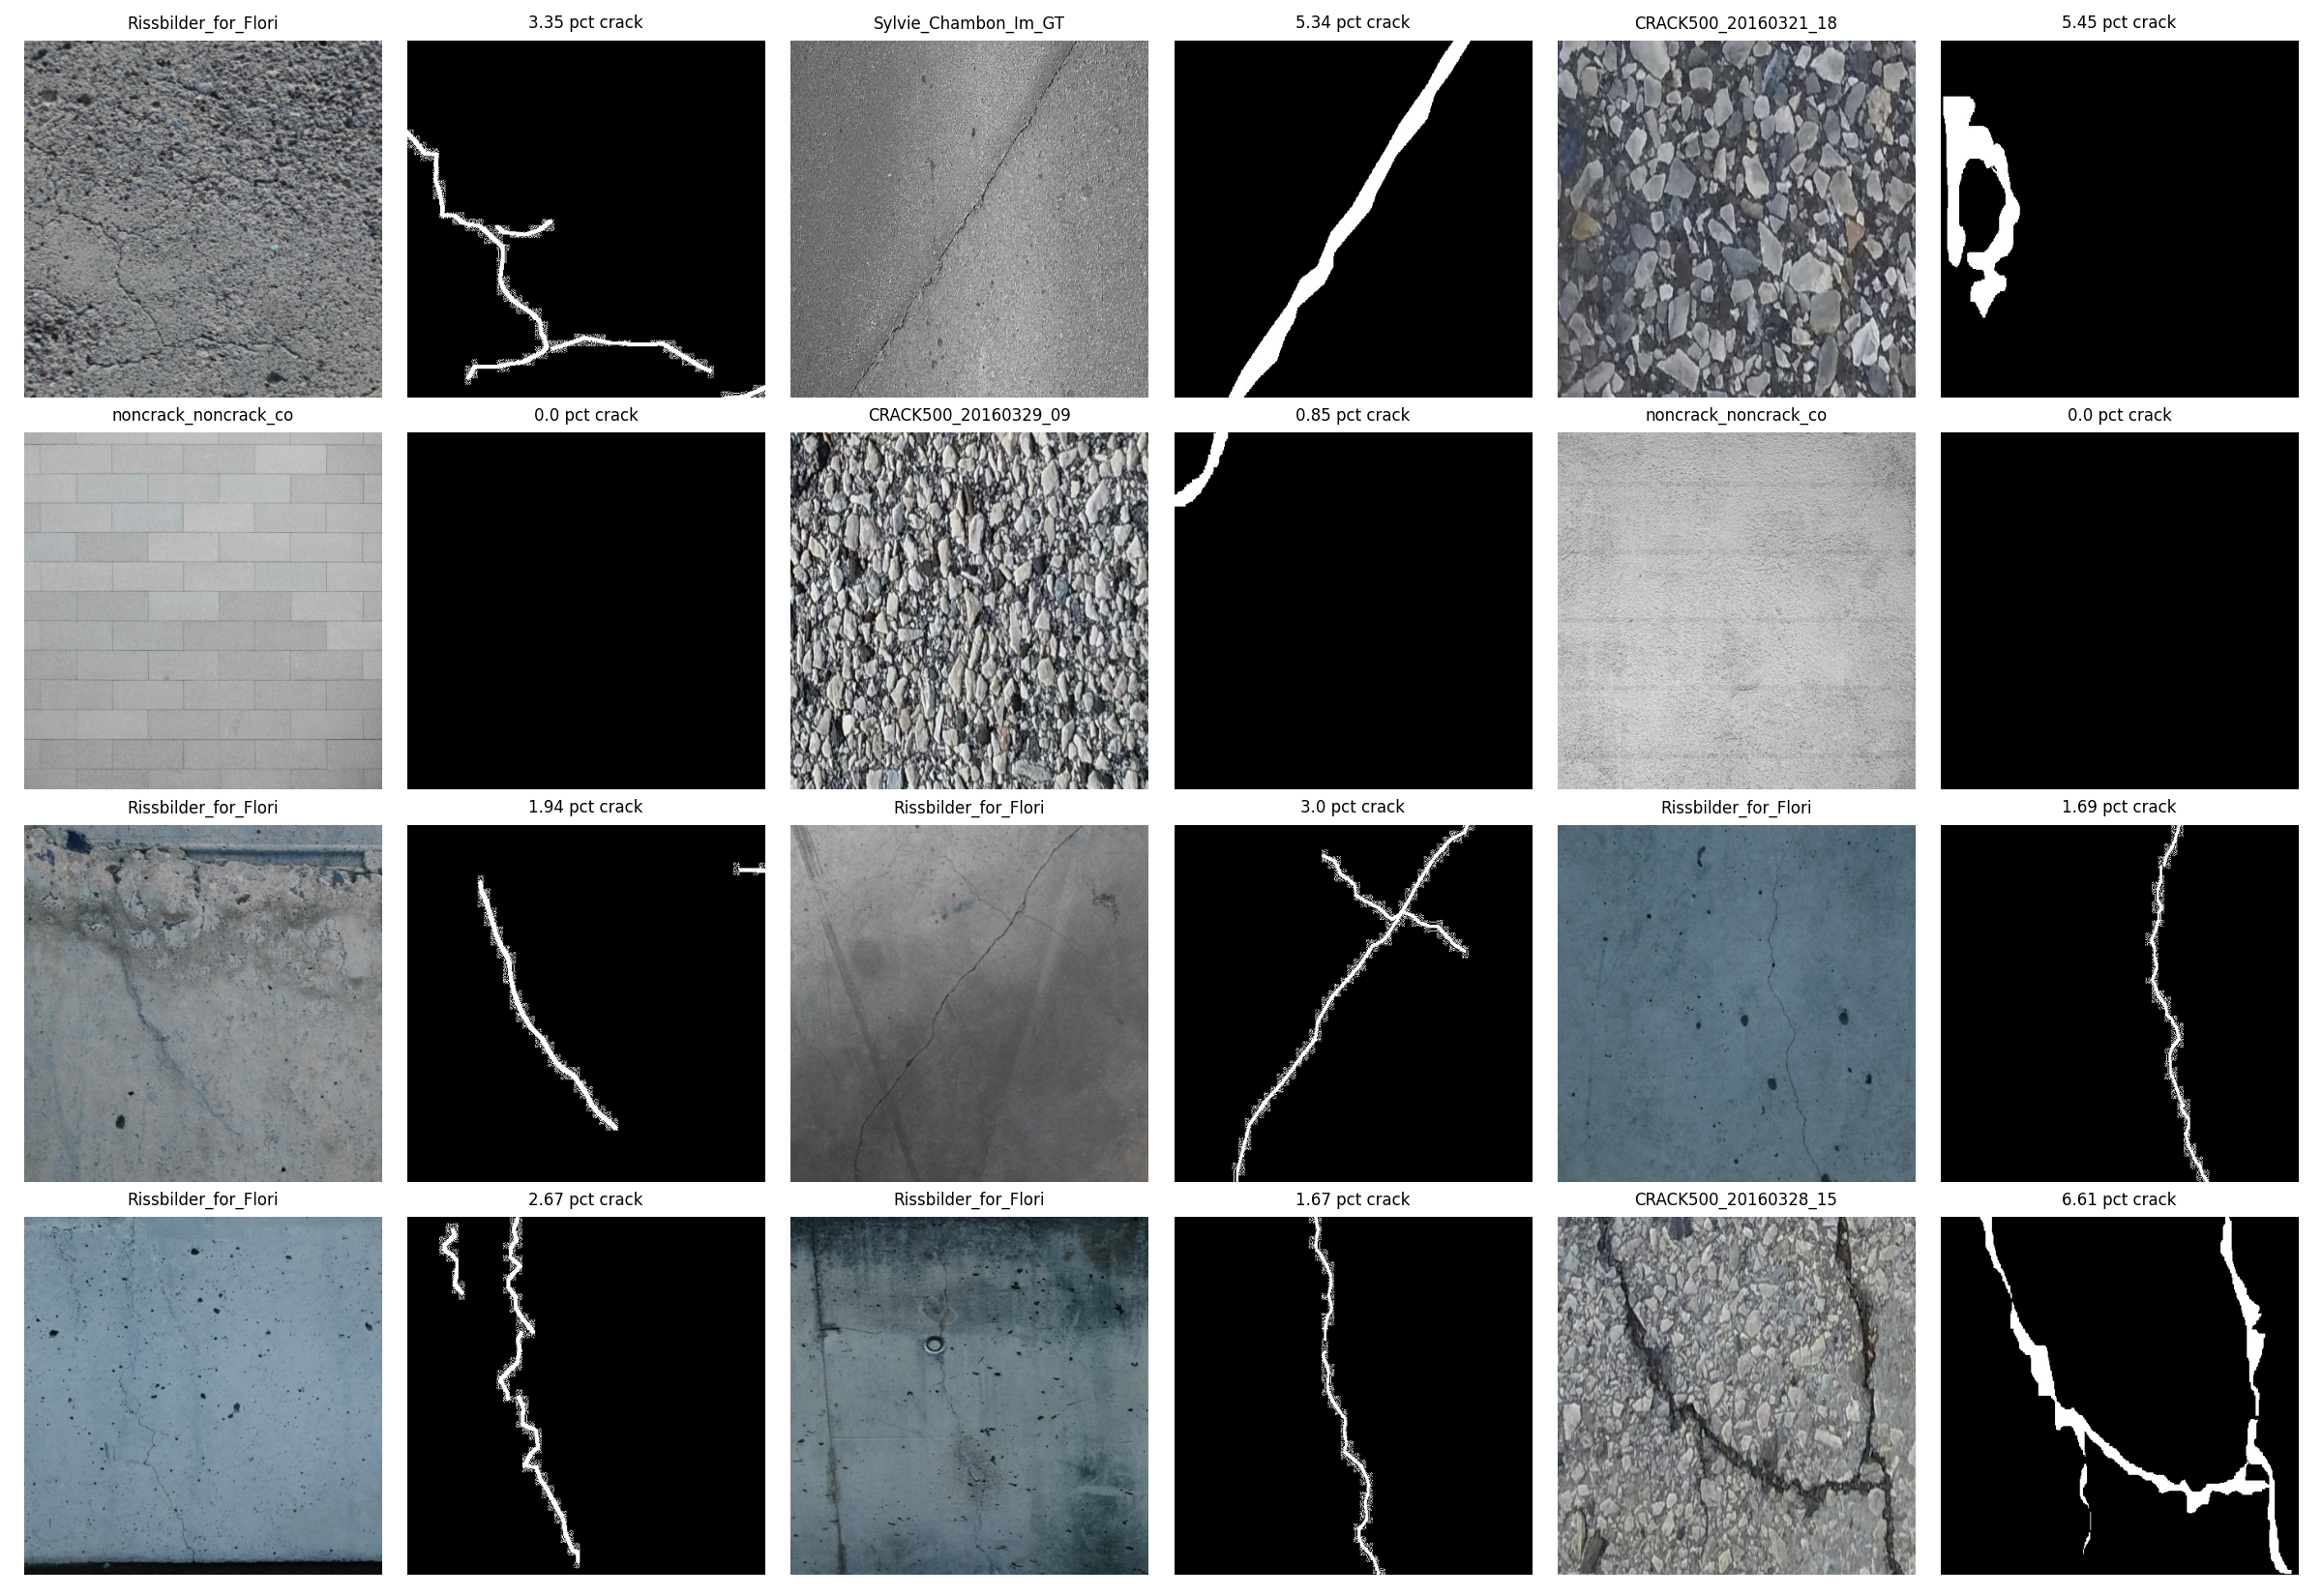
\includegraphics[width=0.9\columnwidth]{audit_samples.png}
\caption{Twelve image and mask pairs from the audit sample. The title above each mask gives its crack pixel percentage.}
\label{fig:samples}
\end{figure}

\begin{figure}[t]
\centering
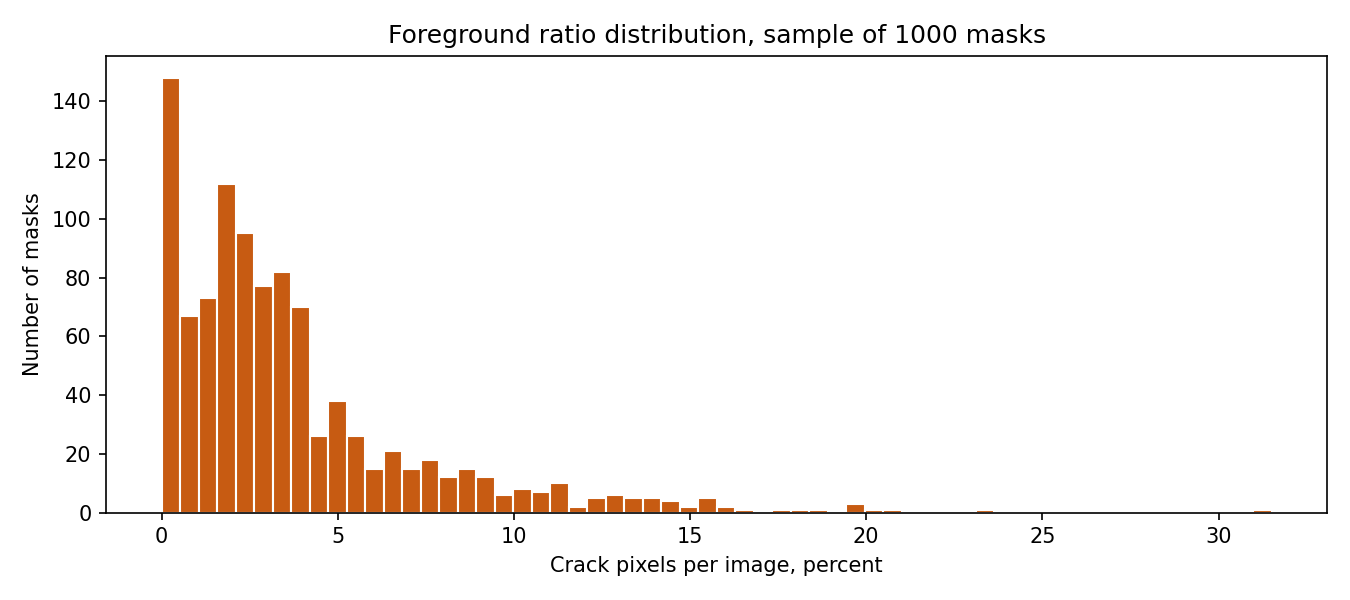
\includegraphics[width=0.85\columnwidth]{foreground_histogram.png}
\caption{Distribution of crack pixel percentage across 1,000 sampled masks.}
\label{fig:hist}
\end{figure}

\subsection{Metrics}
Four metrics are reported for every run. Predictions are thresholded at 0.5. TP, FP and FN count crack pixels that are correctly predicted, wrongly predicted and missed, summed over all test images. The metrics are pooled over all test pixels and are not averaged per image. Their formulas are given in Eqs.~\eqref{eq:dice} to \eqref{eq:recall}.
\begin{align}
\mathrm{Dice}&=\frac{2\,\mathrm{TP}+\epsilon}{2\,\mathrm{TP}+\mathrm{FP}+\mathrm{FN}+\epsilon}\label{eq:dice}\\
\mathrm{IoU}&=\frac{\mathrm{TP}+\epsilon}{\mathrm{TP}+\mathrm{FP}+\mathrm{FN}+\epsilon}\label{eq:iou}\\
\mathrm{Precision}&=\frac{\mathrm{TP}+\epsilon}{\mathrm{TP}+\mathrm{FP}+\epsilon}\label{eq:prec}\\
\mathrm{Recall}&=\frac{\mathrm{TP}+\epsilon}{\mathrm{TP}+\mathrm{FN}+\epsilon}\label{eq:recall}
\end{align}
\noindent where $\epsilon=10^{-6}$ is a smoothing constant. Dice is the primary metric. Precision and recall expose the trade-off between false alarms and missed cracks. An empty ground truth with an empty prediction scores 1.0 for an individual image through $\epsilon$.

\subsection{Implementation Details}
Experiments ran on Google Colab with an NVIDIA Tesla T4 (15,360 MiB) and TensorFlow 2.20.0 with Keras. Mixed precision float16 runs roughly two times faster on the T4 tensor cores. Batch size is 48, the largest that fits ResNet50-UNet at $128\times128$ crops with mixed precision on this GPU. ReduceLROnPlateau halves the learning rate after 2 epochs without a gain in validation Dice, down to a minimum of $10^{-6}$. EarlyStopping ends a run after 4 epochs without a gain and restores the best weights. Validation uses a subset of at most 320 images, and the default seed is 42.

\subsection{Baseline and Comparisons}
The scratch U-Net is the in-study baseline. CoreDeep is the closest prior work because it uses the identical dataset and official split \cite{coredeep}. It reports mIoU gains over baseline methods, and its Dice is not used here \cite{coredeep}. The comparison with CoreDeep is qualitative. The contribution of this study is the ablation and the generalization study, not a higher Dice. DeepCrack and CrackSeg9k serve as related work only, since their data differ \cite{deepcrack,crackseg9k}.

\section{Results and Discussion}
\label{sec:results}
\subsection{Encoder Comparison}
Table~\ref{tab:ablation} lists the runs on Protocol A. VGG16-UNet reaches a Dice of 0.6707 against 0.5980 for the scratch U-Net, a gain of 0.073. IoU rises from 0.4265 to 0.5045, and precision and recall rise from 0.5632 and 0.6373 to 0.6437 and 0.6999. ImageNet pretraining transfers to near-grayscale crack texture in this setting. The backbone swap follows the conversion of classification networks into dense predictors \cite{fcn}. ResNet50-UNet reaches only 0.2246, and Section~\ref{sec:dynamics} examines that result.

\begin{table}[t]
\caption{Ablation on Protocol A (1,647 test images, pooled metrics). E1 and E2 repeat A2 with seeds 101 and 202.}
\label{tab:ablation}
\centering
\scriptsize
\setlength{\tabcolsep}{2.5pt}
\begin{tabular}{llllcccc}
\toprule
Run & Encoder & Loss & Input & Dice & IoU & Prec. & Rec. \\
\midrule
A1 & U-Net & Dice & raw & 0.5980 & 0.4265 & 0.5632 & 0.6373 \\
A2 & VGG16-UNet & Dice & raw & 0.6707 & 0.5045 & 0.6437 & 0.6999 \\
A3 & ResNet50-UNet & Dice & raw & 0.2246 & 0.1265 & 0.1351 & 0.6674 \\
\midrule
B1 & VGG16-UNet & BCE & raw & 0.6436 & 0.4745 & 0.6807 & 0.6104 \\
B2 & VGG16-UNet & Tversky & raw & 0.6651 & 0.4983 & 0.5905 & 0.7613 \\
\midrule
C1 & VGG16-UNet & Dice & CLAHE & 0.6317 & 0.4617 & 0.5747 & 0.7012 \\
C2 & VGG16-UNet & Dice & edge & 0.6538 & 0.4856 & 0.6228 & 0.6880 \\
\midrule
E1 & VGG16-UNet & Dice & raw & 0.6650 & 0.4981 & 0.6484 & 0.6825 \\
E2 & VGG16-UNet & Dice & raw & 0.6734 & 0.5076 & 0.6690 & 0.6779 \\
\bottomrule
\end{tabular}
\end{table}

\subsection{Loss Function Comparison}
BCE reaches a Dice of 0.6436, with the highest precision (0.6807) and the lowest recall (0.6104) of the three losses. The V-Net motivation predicts that cross-entropy collapses to the background when the foreground is scarce \cite{vnet}. No collapse occurs at a background to crack ratio of 26.23 to 1. BCE trades recall for precision, and it trails Dice loss by 0.027 Dice. Fig.~\ref{fig:bce} shows similar BCE and Dice masks on four test images. Both losses widen thin cracks and add blobs near thick cracks, and BCE does not predict crack everywhere.

\begin{figure}[t]
\centering
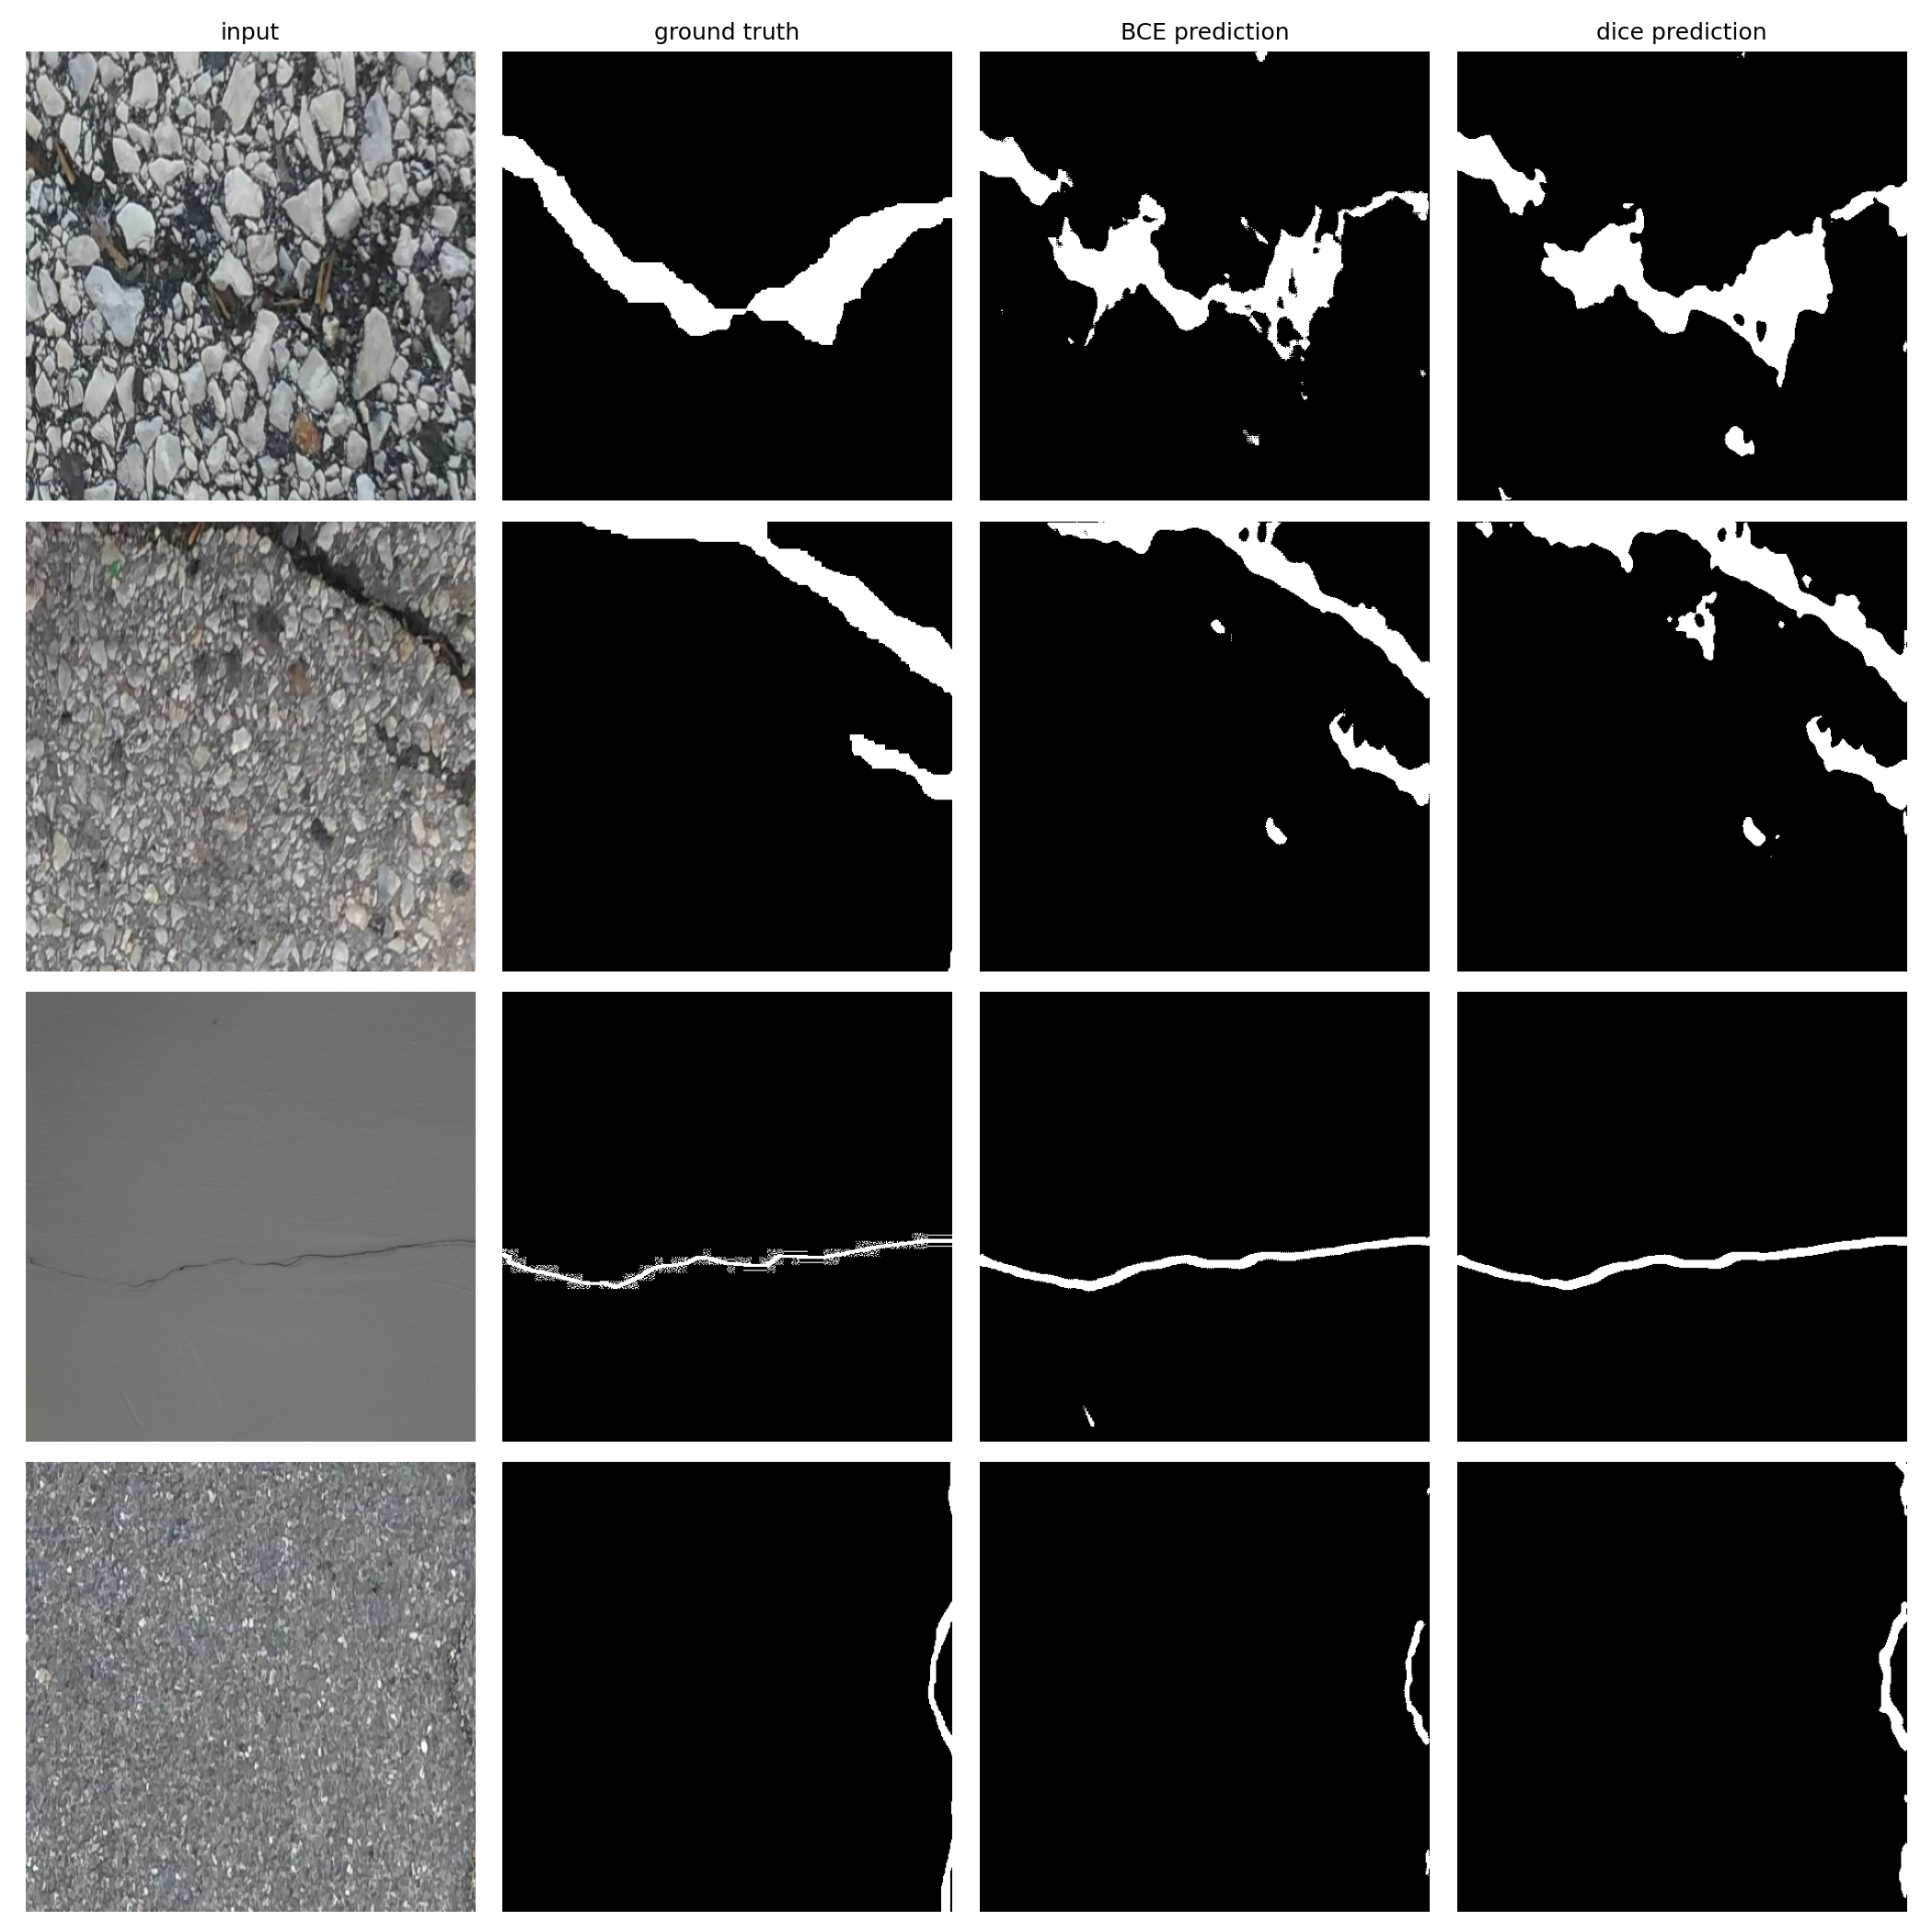
\includegraphics[width=0.62\columnwidth]{fig_bce_failure.png}
\caption{Qualitative loss comparison on four test images. Columns show the input, the ground truth, the BCE prediction and the Dice prediction.}
\label{fig:bce}
\end{figure}

Tversky loss reaches a Dice of 0.6651 with a recall of 0.7613 and a precision of 0.5905. The weight $\beta=0.7$ on false negatives raises recall as designed \cite{tversky}. The Dice values of Dice loss and Tversky loss differ by 0.0056, so the two are comparable in Dice. The operating points differ: Tversky recall is 0.7613 against 0.6999 for Dice loss, and precision is 0.5905 against 0.6437. Structural inspection can prefer the higher recall, because a missed crack costs more than a false alarm.

\subsection{Input Preprocessing}
Raw RGB reaches a Dice of 0.6707, the edge stack 0.6538 and CLAHE 0.6317. The Laplacian channel lowers Dice by 0.017, and CLAHE lowers it by 0.039. Handcrafted edge priors do not help VGG16-UNet at a training size of 7,922 images. A plausible reason is that the encoder learns edge responses from data, which makes an explicit Laplacian channel redundant. The result holds for the VGG16-UNet setting and is not generalized beyond it.

\subsection{Seed Stability and Test Set Leakage}
Stage E repeats the best configuration with seeds 101 and 202. Test Dice is 0.6707, 0.6650 and 0.6734 for seeds 42, 101 and 202. Validation Dice has a mean of 0.6342 and a standard deviation of 0.0043 across the three seeds. The deviation comes from validation scores, and only the best configuration was repeated. Ablation gaps below 0.004 are not claimed as meaningful. The encoder gap of 0.073, the BCE gap of 0.027 and the preprocessing gaps of 0.017 and 0.039 exceed this level.

The official test set holds 48 images that are exact copies of training images, which is 2.83 percent of its 1,695 images. Removing them changes the pooled Dice of model A2 from 0.6633 to 0.6707, a change of +0.0074, and IoU from 0.4962 to 0.5045. The official set with the leaked images scores lower for this model. The measured effect is small, it comes from one model, and the available data does not explain its direction. The leaked images remain a benchmark validity issue, because test images should not appear in training. Results that use the official split contain these images \cite{coredeep}.

\subsection{Cross-Surface Generalization}
Table~\ref{tab:gen} reports the surface-held-out runs. Holding out wall gives a Dice of 0.1704, and holding out pavement gives 0.2103. The size-matched control, trained on 4,054 random images that mix all surface types, reaches 0.6611. The gaps to the control are 0.4907 for wall and 0.4508 for pavement. The control and D1 share a training size of 4,054 images, and D2 trains on 4,578 images. Data volume does not explain the gaps, and they are attributed to domain shift.

\begin{table}[t]
\caption{Cross-surface generalization with VGG16-UNet, Dice loss and raw input. D1 and D2 hold out wall and pavement, and D3 is the size-matched control. Test sets hold 4,864, 4,248 and 4,864 images. Gap is the Dice difference to D3.}
\label{tab:gen}
\centering
\scriptsize
\setlength{\tabcolsep}{2.5pt}
\begin{tabular}{llccccc}
\toprule
Run & Train & Dice & IoU & Prec. & Rec. & Gap \\
\midrule
D1 no wall & 4,054 & 0.1704 & 0.0931 & 0.5292 & 0.1016 & 0.4907 \\
D2 no pavement & 4,578 & 0.2103 & 0.1175 & 0.5718 & 0.1289 & 0.4508 \\
D3 control & 4,054 & 0.6611 & 0.4938 & 0.6424 & 0.6810 & baseline \\
\bottomrule
\end{tabular}
\end{table}

Precision on D1 and D2 is moderate at 0.5292 and 0.5718. Recall collapses to 0.1016 and 0.1289. The model predicts few crack pixels on the unseen surface. About half of the pixels it marks match the masks, and most cracks go undetected. The model learned crack appearance on the seen surfaces and does not carry it to the held-out family.

Table~\ref{tab:family} reports Dice by family for model A2, which saw all families in training. Wall scores 0.6337, pavement 0.6971 and mixed 0.7165. Wall is not intrinsically hard, since it scores 0.6337 when wall images are in training. The low D1 score is consistent with missing wall data in training and not with wall being hard. The claim goes no further, because the two protocols use different test populations.

\begin{table}[t]
\caption{Dice by surface family for model A2 on the deduplicated Protocol A test set, crack images only.}
\label{tab:family}
\centering
\scriptsize
\setlength{\tabcolsep}{3pt}
\begin{tabular}{lccccc}
\toprule
Family & $n$ & Dice & IoU & Prec. & Rec. \\
\midrule
Wall & 728 & 0.6337 & 0.4638 & 0.6569 & 0.6122 \\
Pavement & 638 & 0.6971 & 0.5351 & 0.6581 & 0.7411 \\
Mixed & 78 & 0.7165 & 0.5583 & 0.5945 & 0.9017 \\
\bottomrule
\end{tabular}
\end{table}

\subsection{Qualitative Analysis}
Fig.~\ref{fig:bestworst} shows the four worst and four best cases among 300 sampled test images. All four worst cases score a Dice of 0.0. They are thin cracks on dark or blurred asphalt, and the model predicts almost no crack pixels there. The best cases with a detected crack score from 0.894 to 0.929 and show wide cracks on pavement and concrete. The bottom-right case scores 1.0 because both masks are empty, and it is not a detected crack.

\begin{figure}[t]
\centering
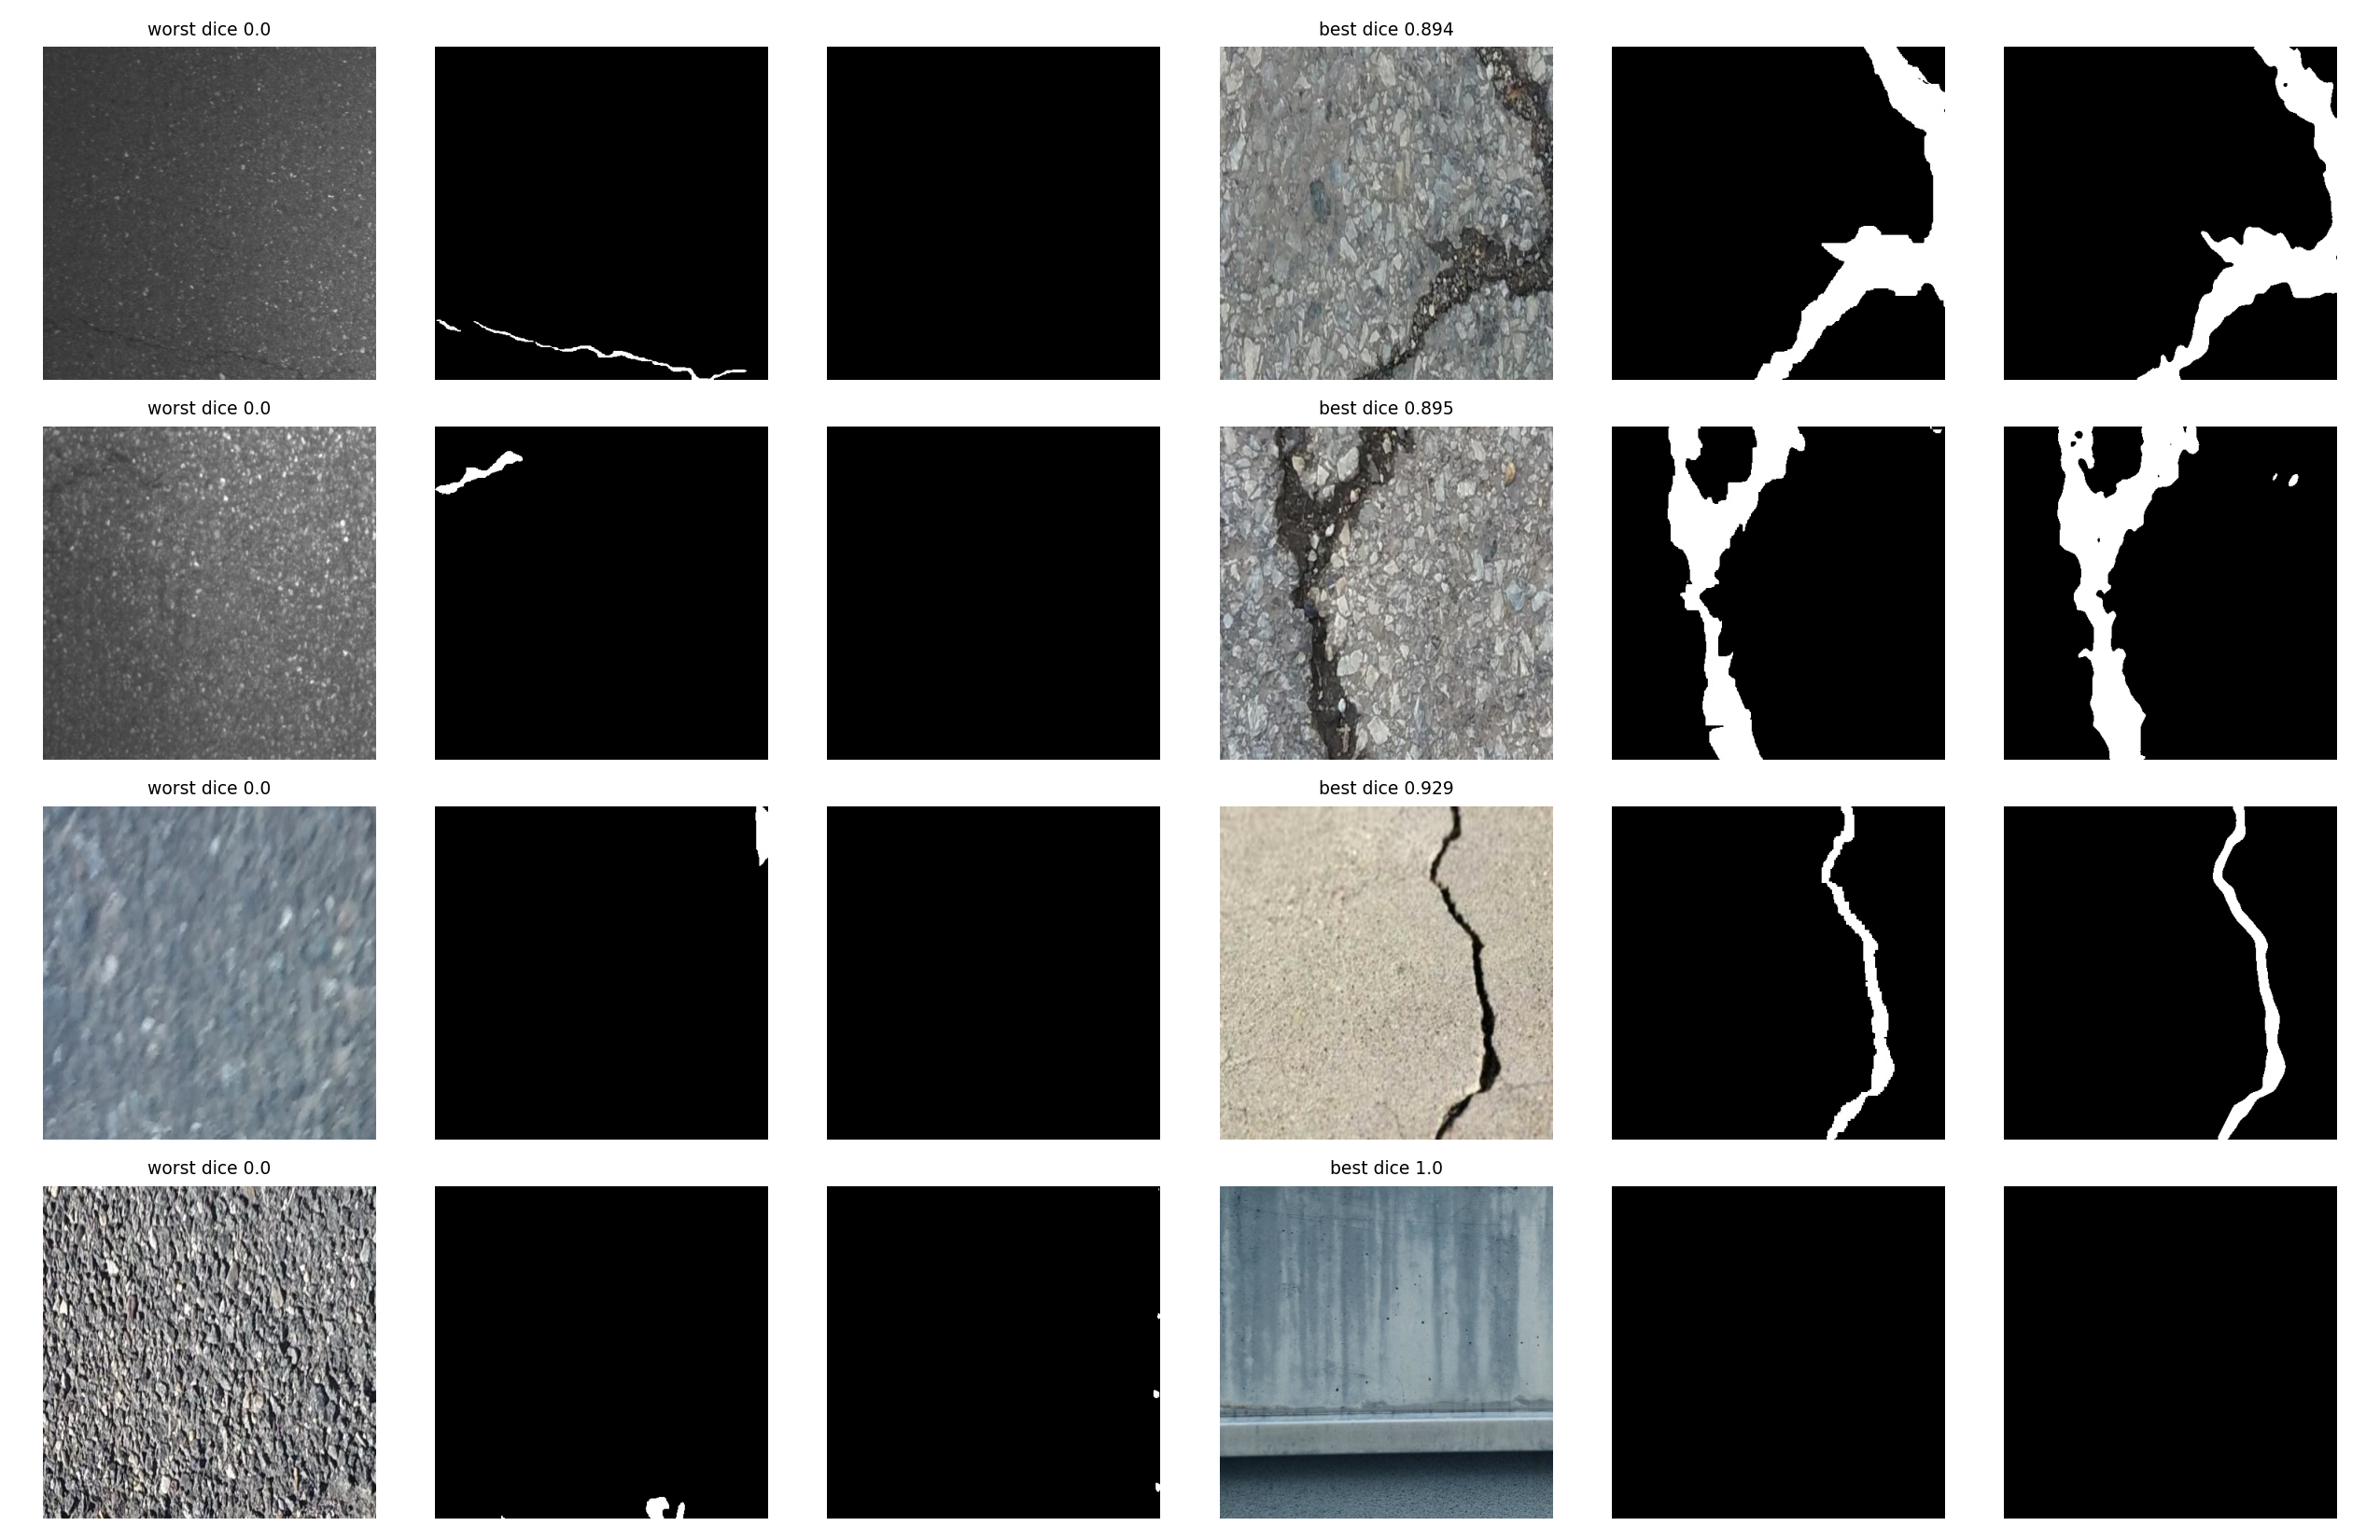
\includegraphics[width=0.95\columnwidth]{fig_best_worst.png}
\caption{Four worst and four best cases by Dice among 300 sampled test images. Left triplets show the worst cases and right triplets the best cases, each as input, ground truth and prediction. The bottom-right best case has an empty ground truth and an empty prediction. It scores 1.0 through the smoothing term and is not a detected crack.}
\label{fig:bestworst}
\end{figure}

\subsection{Training Dynamics}
\label{sec:dynamics}
Fig.~\ref{fig:curves} shows validation Dice by epoch for A1, A2, A3 and B1. ResNet50-UNet peaks at about 0.22 in epoch 3, the last epoch with a frozen encoder. Its validation Dice falls to 0.0 in epochs 4 to 6 after the encoder is unfrozen, and early stopping ends the run at epoch 7. The reported ResNet50 result is the epoch 3 checkpoint, before any encoder fine-tuning. VGG16-UNet also dips in epoch 4 and recovers to its peak of 0.6351 in epoch 8. The scratch U-Net and the BCE run stay below that peak.

\begin{figure}[t]
\centering
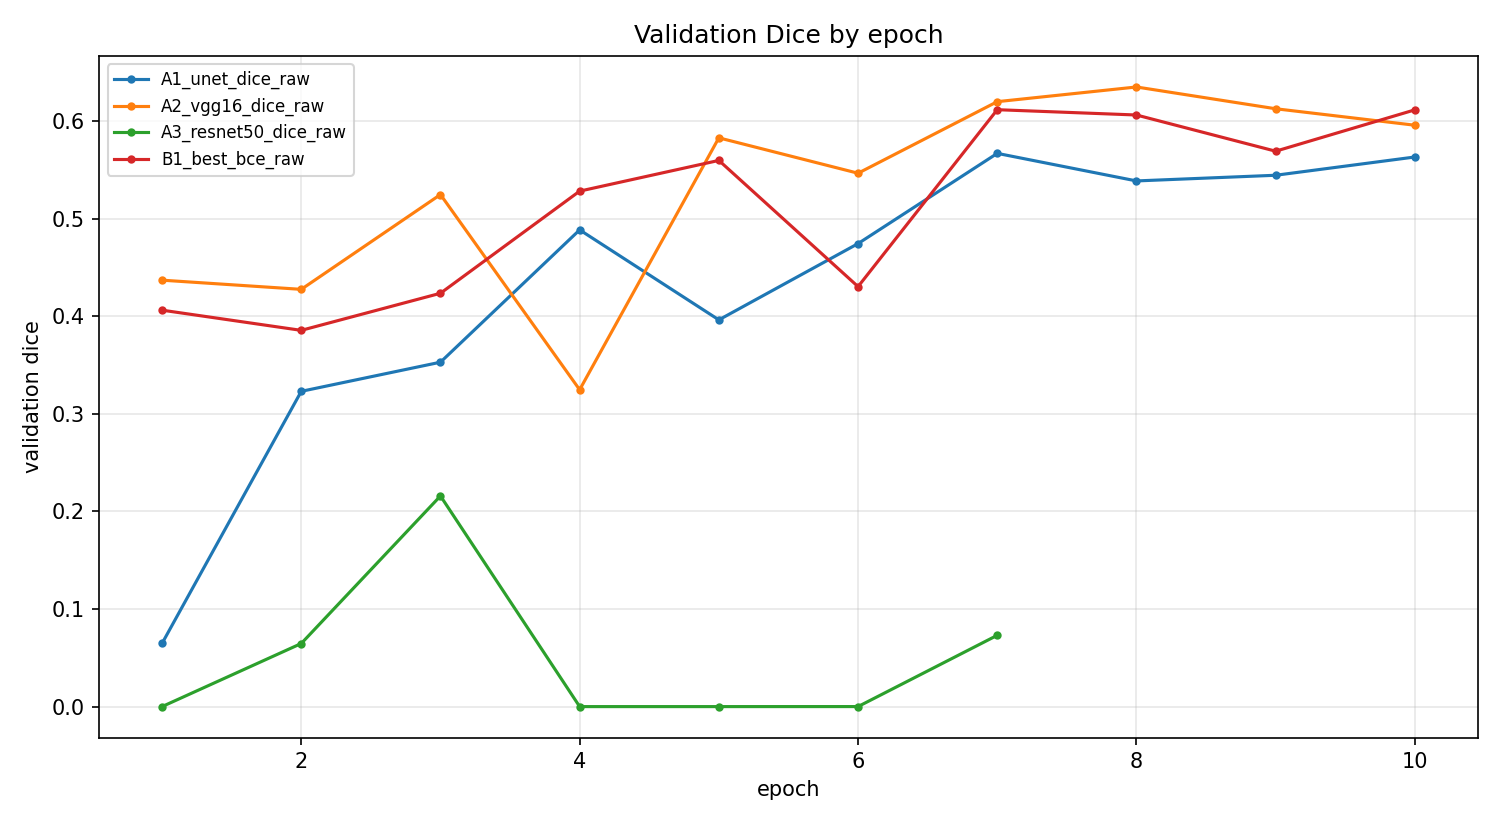
\includegraphics[width=0.92\columnwidth]{fig_training_curves.png}
\caption{Validation Dice by epoch for A1, A2, A3 and B1. The ResNet50-UNet run (A3) stops at epoch 7.}
\label{fig:curves}
\end{figure}

The collapse follows unfreezing, and the run stopped at about 1,050 updates. The step budget of 1,500 updates does not explain the collapse, because the run never used the full budget. The cause is untested. Section~\ref{sec:limits} names three candidate causes.

\section{Limitations and Threats to Validity}
\label{sec:limits}
The ResNet50 result is an epoch 3 checkpoint, and the cause of the collapse is untested. Three candidate causes remain: unfreezing at learning rate $10^{-4}$, BatchNorm layers becoming trainable at batch 48, and input scaling to 0 to 1 instead of the backbone's native preprocessing. The Tversky weight $\beta=0.7$ was set by domain reasoning and not by search. No transformer backbone and no CRF post-processing were tested. The threshold is fixed at 0.5 for all runs, and an oracle threshold was not computed. Each ablation run uses one seed, and the seed deviation of 0.0043 comes from validation scores of the best configuration only.

The merged dataset is not annotation-cleaned, and CrackSeg9k raised annotation problems for its constituent datasets \cite{crackseg9k}. Only two surface families were held out, and family labels come from filename prefixes. The mixed family holds 521 images from one source prefix and appears in every Protocol B training set. The leakage effect was measured on one model only. Protocol A test data include crack-free images and Protocol B test data do not, so absolute scores are not comparable across protocols.

\section{Conclusion and Future Work}
\label{sec:conclusion}
This study measured the effect of encoder, loss and preprocessing on crack segmentation and the effect of an unseen surface type. VGG16-UNet with Dice loss and raw RGB input reaches a test Dice of 0.6707 on the deduplicated official split, and 0.6734 with seed 202. BCE does not collapse, and handcrafted edge and CLAHE inputs do not help. Holding out a surface family lowers Dice to 0.1704 for wall and 0.2103 for pavement, against 0.6611 for a size-matched control. The audit found 331 duplicates, 48 leaked test images and aliased source prefixes.

Future work will isolate the cause of the ResNet50 collapse by testing the three candidate causes. A search over the Tversky weights can test whether recall improves further. Transformer backbones and CRF post-processing are candidates for later study. More held-out families and more seeds for each ablation run would tighten the estimates.

\section*{Acknowledgment}
This work was completed for CSE463 Computer Vision, Section 03, Summer 2026, BRAC University, under Dr. Md. Ashraful Alam.

\begin{thebibliography}{10}

\bibitem{fcn}
J. Long, E. Shelhamer, and T. Darrell, "Fully convolutional networks for semantic segmentation," in Proc. IEEE Conf. Computer Vision and Pattern Recognition (CVPR), 2015, pp. 3431-3440.

\bibitem{unet}
O. Ronneberger, P. Fischer, and T. Brox, "U-Net: Convolutional networks for biomedical image segmentation," in Proc. Medical Image Computing and Computer-Assisted Intervention (MICCAI), 2015, arXiv:1505.04597.

\bibitem{deepcrack}
Y. Liu, J. Yao, X. Lu, R. Xie, and L. Li, "DeepCrack: A deep hierarchical feature learning architecture for crack segmentation," Neurocomputing, vol. 338, pp. 139-153, 2019, doi: 10.1016/j.neucom.2019.01.036.

\bibitem{coredeep}
P. Nagrath et al., "CoreDeep: Improving crack detection algorithms using width stochasticity," arXiv preprint arXiv:2209.04648, 2022.

\bibitem{crackseg9k}
S. Kulkarni et al., "CrackSeg9k: A collection and benchmark for crack segmentation datasets and frameworks," in Proc. ECCV Workshops, 2022, LNCS 13807, pp. 179-195.

\bibitem{segnet}
V. Badrinarayanan, A. Kendall, and R. Cipolla, "SegNet: A deep convolutional encoder-decoder architecture for image segmentation," IEEE Trans. Pattern Anal. Mach. Intell., vol. 39, no. 12, pp. 2481-2495, 2017.

\bibitem{deeplab}
L.-C. Chen, Y. Zhu, G. Papandreou, F. Schroff, and H. Adam, "Encoder-decoder with atrous separable convolution for semantic image segmentation," in Proc. European Conf. Computer Vision (ECCV), 2018, arXiv:1802.02611.

\bibitem{vnet}
F. Milletari, N. Navab, and S.-A. Ahmadi, "V-Net: Fully convolutional neural networks for volumetric medical image segmentation," in Proc. Int. Conf. 3D Vision (3DV), 2016, arXiv:1606.04797.

\bibitem{tversky}
S. S. M. Salehi, D. Erdogmus, and A. Gholipour, "Tversky loss function for image segmentation using 3D fully convolutional deep networks," in Proc. MLMI Workshop, MICCAI, 2017, arXiv:1706.05721.

\bibitem{attnunet}
O. Oktay et al., "Attention U-Net: Learning where to look for the pancreas," in Proc. Medical Imaging with Deep Learning (MIDL), 2018, arXiv:1804.03999.

\end{thebibliography}

\end{document}
